\documentclass{standalone}
\usepackage{tikz}
\usetikzlibrary{patterns}
\usetikzlibrary{positioning}
\usetikzlibrary{patterns, positioning}
\usetikzlibrary{shapes.misc}
\usepackage[outline]{contour}
\contourlength{1.5pt} 
\usetikzlibrary{calc}
        \usepackage{relsize}
        \tikzset{fontscale/.style = {font=\relsize{#1}}}

\begin{document}
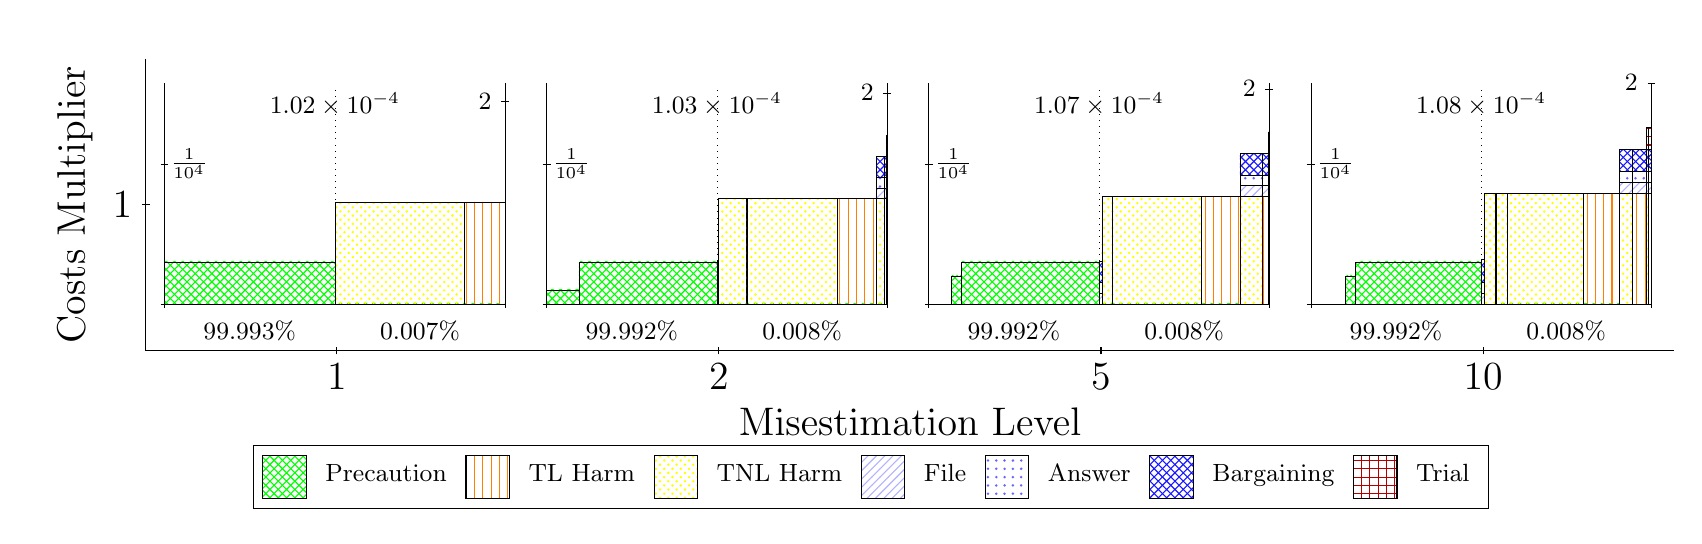
\begin{tikzpicture}
\clip(-0.5,-1.1) rectangle +(20.91,6.2);
\draw[black] (1,1) -- (1,4.7);
\node[rotate=90, fontscale=2, anchor=center] at (0.1, 2.85) {Costs Multiplier};
\draw[black] (0.95,2.85) -- (1.05,2.85);
\node[fontscale=2, anchor=east] at (0.95, 2.85) {1};

\draw[black] (1,1) -- (20.41,1);
\node[fontscale=2, anchor=center] at (10.705, 0.1) {Misestimation Level};
\draw[black] (3.4263,0.95) -- (3.4263,1.05);
\node[fontscale=2, anchor=north] at (3.4263, 0.95) {1};
\draw[black] (8.2788,0.95) -- (8.2788,1.05);
\node[fontscale=2, anchor=north] at (8.2788, 0.95) {2};
\draw[black] (13.131,0.95) -- (13.131,1.05);
\node[fontscale=2, anchor=north] at (13.131, 0.95) {5};
\draw[black] (17.984,0.95) -- (17.984,1.05);
\node[fontscale=2, anchor=north] at (17.984, 0.95) {10};


\draw[pattern=crosshatch, pattern color=green,draw=black,very thin] (1.2381,1.592) rectangle (3.4013,2.1252);
\draw[pattern=crosshatch, pattern color=green,draw=black,very thin] (3.4013,1.592) rectangle (5.0472,1.592);
\draw[pattern=crosshatch dots, pattern color=yellow,draw=black,very thin] (3.4013,1.592) rectangle (5.0472,2.8791);
\draw[pattern=crosshatch, pattern color=green,draw=black,very thin] (5.0472,1.592) rectangle (5.5644,1.592);
\draw[pattern=vertical lines, pattern color=orange,draw=black,very thin] (5.0472,1.592) rectangle (5.5644,2.8791);
\node[font=\small,text=black,anchor=north] at (3.4013, 4.4) {$1.02\times 10^{-4}$};
\draw[black,very thin] (1.2381,1.592) -- (1.2381,4.4);
\draw[black,very thin] (1.1881,1.592) -- (1.2881,1.592);
\node[font=\small,text=black, anchor=west] at (1.1881, 1.592) {};
\draw[black,very thin] (1.1881,3.3694) -- (1.2881,3.3694);
\node[font=\small,text=black, anchor=west] at (1.1881, 3.3694) {$\frac{1}{10^{4}}$};

\draw[black,dotted,very thin] (3.4013,1.6762) -- (3.4013,4.3158);
\draw[black,very thin] (5.5644,1.592) -- (5.5644,4.4);
\draw[black,very thin] (5.5144,4.1662) -- (5.6144,4.1662);
\node[font=\small,text=black, anchor=east] at (5.5144, 4.1662) {\contour{white}{2}};

\draw[black,very thin] (1.2381,1.592) -- (5.5644,1.592);
\draw[black,very thin] (1.2381,1.542) -- (1.2381,1.642);
\node[font=\small,text=black, anchor=north] at (1.2381, 1.542) {};
\draw[black,very thin] (5.5644,1.542) -- (5.5644,1.642);
\node[font=\small,text=black, anchor=north] at (5.5644, 1.542) {};

\node[font=\small,text=black,anchor=south] at (2.3197, 0.992) {99.993\%};
\node[font=\small,text=black,anchor=south] at (4.4828, 0.992) {0.007\%};

\draw[pattern=crosshatch, pattern color=green,draw=black,very thin] (6.0906,1.592) rectangle (6.5013,1.7697);
\draw[pattern=crosshatch, pattern color=green,draw=black,very thin] (6.5013,1.592) rectangle (8.2538,2.1252);
\draw[pattern=crosshatch, pattern color=green,draw=black,very thin] (8.2538,1.592) rectangle (8.2669,1.592);
\draw[pattern=north east lines, pattern color=blue!30,draw=black,very thin] (8.2538,1.592) rectangle (8.2669,1.726);
\draw[pattern=dots,  pattern color=blue!60,draw=black,very thin] (8.2538,1.726) rectangle (8.2669,1.86);
\draw[pattern=crosshatch,      pattern color=blue!90,draw=black,very thin] (8.2538,1.86) rectangle (8.2669,2.128);
\draw[pattern=crosshatch, pattern color=green,draw=black,very thin] (8.2669,1.592) rectangle (8.2687,1.592);
\draw[pattern=north east lines, pattern color=blue!30,draw=black,very thin] (8.2669,1.592) rectangle (8.2687,1.726);
\draw[pattern=dots,  pattern color=blue!60,draw=black,very thin] (8.2669,1.726) rectangle (8.2687,1.86);
\draw[pattern=crosshatch,      pattern color=blue!90,draw=black,very thin] (8.2669,1.86) rectangle (8.2687,2.128);
\draw[pattern=grid,            pattern color=red!70!black,draw=black,very thin] (8.2669,2.128) rectangle (8.2687,2.396);
\draw[pattern=crosshatch, pattern color=green,draw=black,very thin] (8.2687,1.592) rectangle (8.6301,1.592);
\draw[pattern=crosshatch dots, pattern color=yellow,draw=black,very thin] (8.2687,1.592) rectangle (8.6301,2.932);
\draw[pattern=crosshatch, pattern color=green,draw=black,very thin] (8.6301,1.592) rectangle (8.6351,1.592);
\draw[pattern=vertical lines, pattern color=orange,draw=black,very thin] (8.6301,1.592) rectangle (8.6351,2.932);
\draw[pattern=crosshatch, pattern color=green,draw=black,very thin] (8.6351,1.592) rectangle (9.7867,1.592);
\draw[pattern=crosshatch dots, pattern color=yellow,draw=black,very thin] (8.6351,1.592) rectangle (9.7867,2.932);
\draw[pattern=crosshatch, pattern color=green,draw=black,very thin] (9.7867,1.592) rectangle (10.281,1.592);
\draw[pattern=vertical lines, pattern color=orange,draw=black,very thin] (9.7867,1.592) rectangle (10.281,2.932);
\draw[pattern=crosshatch, pattern color=green,draw=black,very thin] (10.281,1.592) rectangle (10.373,1.592);
\draw[pattern=crosshatch dots, pattern color=yellow,draw=black,very thin] (10.281,1.592) rectangle (10.373,2.932);
\draw[pattern=north east lines, pattern color=blue!30,draw=black,very thin] (10.281,2.932) rectangle (10.373,3.066);
\draw[pattern=dots,  pattern color=blue!60,draw=black,very thin] (10.281,3.066) rectangle (10.373,3.2);
\draw[pattern=crosshatch,      pattern color=blue!90,draw=black,very thin] (10.281,3.2) rectangle (10.373,3.468);
\draw[pattern=crosshatch, pattern color=green,draw=black,very thin] (10.373,1.592) rectangle (10.401,1.592);
\draw[pattern=vertical lines, pattern color=orange,draw=black,very thin] (10.373,1.592) rectangle (10.401,2.932);
\draw[pattern=north east lines, pattern color=blue!30,draw=black,very thin] (10.373,2.932) rectangle (10.401,3.066);
\draw[pattern=dots,  pattern color=blue!60,draw=black,very thin] (10.373,3.066) rectangle (10.401,3.2);
\draw[pattern=crosshatch,      pattern color=blue!90,draw=black,very thin] (10.373,3.2) rectangle (10.401,3.468);
\draw[pattern=crosshatch, pattern color=green,draw=black,very thin] (10.401,1.592) rectangle (10.413,1.592);
\draw[pattern=crosshatch dots, pattern color=yellow,draw=black,very thin] (10.401,1.592) rectangle (10.413,2.932);
\draw[pattern=north east lines, pattern color=blue!30,draw=black,very thin] (10.401,2.932) rectangle (10.413,3.066);
\draw[pattern=dots,  pattern color=blue!60,draw=black,very thin] (10.401,3.066) rectangle (10.413,3.2);
\draw[pattern=crosshatch,      pattern color=blue!90,draw=black,very thin] (10.401,3.2) rectangle (10.413,3.468);
\draw[pattern=grid,            pattern color=red!70!black,draw=black,very thin] (10.401,3.468) rectangle (10.413,3.736);
\draw[pattern=crosshatch, pattern color=green,draw=black,very thin] (10.413,1.592) rectangle (10.417,1.592);
\draw[pattern=vertical lines, pattern color=orange,draw=black,very thin] (10.413,1.592) rectangle (10.417,2.932);
\draw[pattern=north east lines, pattern color=blue!30,draw=black,very thin] (10.413,2.932) rectangle (10.417,3.066);
\draw[pattern=dots,  pattern color=blue!60,draw=black,very thin] (10.413,3.066) rectangle (10.417,3.2);
\draw[pattern=crosshatch,      pattern color=blue!90,draw=black,very thin] (10.413,3.2) rectangle (10.417,3.468);
\draw[pattern=grid,            pattern color=red!70!black,draw=black,very thin] (10.413,3.468) rectangle (10.417,3.736);
\node[font=\small,text=black,anchor=north] at (8.2538, 4.4) {$1.03\times 10^{-4}$};
\draw[black,very thin] (6.0906,1.592) -- (6.0906,4.4);
\draw[black,very thin] (6.0406,1.592) -- (6.1406,1.592);
\node[font=\small,text=black, anchor=west] at (6.0406, 1.592) {};
\draw[black,very thin] (6.0406,3.3694) -- (6.1406,3.3694);
\node[font=\small,text=black, anchor=west] at (6.0406, 3.3694) {$\frac{1}{10^{4}}$};

\draw[black,dotted,very thin] (8.2538,1.6762) -- (8.2538,4.3158);
\draw[black,very thin] (10.417,1.592) -- (10.417,4.4);
\draw[black,very thin] (10.367,4.2719) -- (10.467,4.2719);
\node[font=\small,text=black, anchor=east] at (10.367, 4.2719) {\contour{white}{2}};

\draw[black,very thin] (6.0906,1.592) -- (10.417,1.592);
\draw[black,very thin] (6.0906,1.542) -- (6.0906,1.642);
\node[font=\small,text=black, anchor=north] at (6.0906, 1.542) {};
\draw[black,very thin] (10.417,1.542) -- (10.417,1.642);
\node[font=\small,text=black, anchor=north] at (10.417, 1.542) {};

\node[font=\small,text=black,anchor=south] at (7.1722, 0.992) {99.992\%};
\node[font=\small,text=black,anchor=south] at (9.3353, 0.992) {0.008\%};

\draw[pattern=crosshatch, pattern color=green,draw=black,very thin] (11.226,1.592) rectangle (11.354,1.9475);
\draw[pattern=crosshatch, pattern color=green,draw=black,very thin] (11.354,1.592) rectangle (13.106,2.1252);
\draw[pattern=north east lines, pattern color=blue!30,draw=black,very thin] (13.106,1.592) rectangle (13.142,1.7286);
\draw[pattern=dots,  pattern color=blue!60,draw=black,very thin] (13.106,1.7286) rectangle (13.142,1.8651);
\draw[pattern=crosshatch,      pattern color=blue!90,draw=black,very thin] (13.106,1.8651) rectangle (13.142,2.1382);
\draw[pattern=north east lines, pattern color=blue!30,draw=black,very thin] (13.142,1.592) rectangle (13.143,1.7286);
\draw[pattern=dots,  pattern color=blue!60,draw=black,very thin] (13.142,1.7286) rectangle (13.143,1.8651);
\draw[pattern=crosshatch,      pattern color=blue!90,draw=black,very thin] (13.142,1.8651) rectangle (13.143,2.1382);
\draw[pattern=grid,            pattern color=red!70!black,draw=black,very thin] (13.142,2.1382) rectangle (13.143,2.4114);
\draw[pattern=crosshatch, pattern color=green,draw=black,very thin] (13.143,1.592) rectangle (13.279,1.592);
\draw[pattern=crosshatch dots, pattern color=yellow,draw=black,very thin] (13.143,1.592) rectangle (13.279,2.9577);
\draw[pattern=crosshatch, pattern color=green,draw=black,very thin] (13.279,1.592) rectangle (14.409,1.592);
\draw[pattern=crosshatch dots, pattern color=yellow,draw=black,very thin] (13.279,1.592) rectangle (14.409,2.9577);
\draw[pattern=crosshatch, pattern color=green,draw=black,very thin] (14.409,1.592) rectangle (14.894,1.592);
\draw[pattern=vertical lines, pattern color=orange,draw=black,very thin] (14.409,1.592) rectangle (14.894,2.9577);
\draw[pattern=crosshatch dots, pattern color=yellow,draw=black,very thin] (14.894,1.592) rectangle (15.179,2.9576);
\draw[pattern=north east lines, pattern color=blue!30,draw=black,very thin] (14.894,2.9576) rectangle (15.179,3.0942);
\draw[pattern=dots,  pattern color=blue!60,draw=black,very thin] (14.894,3.0942) rectangle (15.179,3.2307);
\draw[pattern=crosshatch,      pattern color=blue!90,draw=black,very thin] (14.894,3.2307) rectangle (15.179,3.5039);
\draw[pattern=vertical lines, pattern color=orange,draw=black,very thin] (15.179,1.592) rectangle (15.253,2.9576);
\draw[pattern=north east lines, pattern color=blue!30,draw=black,very thin] (15.179,2.9576) rectangle (15.253,3.0942);
\draw[pattern=dots,  pattern color=blue!60,draw=black,very thin] (15.179,3.0942) rectangle (15.253,3.2307);
\draw[pattern=crosshatch,      pattern color=blue!90,draw=black,very thin] (15.179,3.2307) rectangle (15.253,3.5039);
\draw[pattern=crosshatch, pattern color=green,draw=black,very thin] (15.253,1.592) rectangle (15.259,1.592);
\draw[pattern=crosshatch dots, pattern color=yellow,draw=black,very thin] (15.253,1.592) rectangle (15.259,2.9577);
\draw[pattern=north east lines, pattern color=blue!30,draw=black,very thin] (15.253,2.9577) rectangle (15.259,3.0942);
\draw[pattern=dots,  pattern color=blue!60,draw=black,very thin] (15.253,3.0942) rectangle (15.259,3.2308);
\draw[pattern=crosshatch,      pattern color=blue!90,draw=black,very thin] (15.253,3.2308) rectangle (15.259,3.5039);
\draw[pattern=crosshatch, pattern color=green,draw=black,very thin] (15.259,1.592) rectangle (15.26,1.592);
\draw[pattern=vertical lines, pattern color=orange,draw=black,very thin] (15.259,1.592) rectangle (15.26,2.9577);
\draw[pattern=north east lines, pattern color=blue!30,draw=black,very thin] (15.259,2.9577) rectangle (15.26,3.0942);
\draw[pattern=dots,  pattern color=blue!60,draw=black,very thin] (15.259,3.0942) rectangle (15.26,3.2308);
\draw[pattern=crosshatch,      pattern color=blue!90,draw=black,very thin] (15.259,3.2308) rectangle (15.26,3.5039);
\draw[pattern=crosshatch dots, pattern color=yellow,draw=black,very thin] (15.26,1.592) rectangle (15.26,2.9576);
\draw[pattern=north east lines, pattern color=blue!30,draw=black,very thin] (15.26,2.9576) rectangle (15.26,3.0942);
\draw[pattern=dots,  pattern color=blue!60,draw=black,very thin] (15.26,3.0942) rectangle (15.26,3.2307);
\draw[pattern=crosshatch,      pattern color=blue!90,draw=black,very thin] (15.26,3.2307) rectangle (15.26,3.5039);
\draw[pattern=grid,            pattern color=red!70!black,draw=black,very thin] (15.26,3.5039) rectangle (15.26,3.777);
\draw[pattern=vertical lines, pattern color=orange,draw=black,very thin] (15.26,1.592) rectangle (15.268,2.9576);
\draw[pattern=north east lines, pattern color=blue!30,draw=black,very thin] (15.26,2.9576) rectangle (15.268,3.0942);
\draw[pattern=dots,  pattern color=blue!60,draw=black,very thin] (15.26,3.0942) rectangle (15.268,3.2307);
\draw[pattern=crosshatch,      pattern color=blue!90,draw=black,very thin] (15.26,3.2307) rectangle (15.268,3.5039);
\draw[pattern=grid,            pattern color=red!70!black,draw=black,very thin] (15.26,3.5039) rectangle (15.268,3.777);
\draw[pattern=crosshatch, pattern color=green,draw=black,very thin] (15.268,1.592) rectangle (15.269,1.592);
\draw[pattern=crosshatch dots, pattern color=yellow,draw=black,very thin] (15.268,1.592) rectangle (15.269,2.9577);
\draw[pattern=north east lines, pattern color=blue!30,draw=black,very thin] (15.268,2.9577) rectangle (15.269,3.0942);
\draw[pattern=dots,  pattern color=blue!60,draw=black,very thin] (15.268,3.0942) rectangle (15.269,3.2308);
\draw[pattern=crosshatch,      pattern color=blue!90,draw=black,very thin] (15.268,3.2308) rectangle (15.269,3.5039);
\draw[pattern=grid,            pattern color=red!70!black,draw=black,very thin] (15.268,3.5039) rectangle (15.269,3.777);
\draw[pattern=crosshatch, pattern color=green,draw=black,very thin] (15.269,1.592) rectangle (15.269,1.592);
\draw[pattern=vertical lines, pattern color=orange,draw=black,very thin] (15.269,1.592) rectangle (15.269,2.9577);
\draw[pattern=north east lines, pattern color=blue!30,draw=black,very thin] (15.269,2.9577) rectangle (15.269,3.0942);
\draw[pattern=dots,  pattern color=blue!60,draw=black,very thin] (15.269,3.0942) rectangle (15.269,3.2308);
\draw[pattern=crosshatch,      pattern color=blue!90,draw=black,very thin] (15.269,3.2308) rectangle (15.269,3.5039);
\draw[pattern=grid,            pattern color=red!70!black,draw=black,very thin] (15.269,3.5039) rectangle (15.269,3.777);
\node[font=\small,text=black,anchor=north] at (13.106, 4.4) {$1.07\times 10^{-4}$};
\draw[black,very thin] (10.943,1.592) -- (10.943,4.4);
\draw[black,very thin] (10.893,1.592) -- (10.993,1.592);
\node[font=\small,text=black, anchor=west] at (10.893, 1.592) {};
\draw[black,very thin] (10.893,3.3694) -- (10.993,3.3694);
\node[font=\small,text=black, anchor=west] at (10.893, 3.3694) {$\frac{1}{10^{4}}$};

\draw[black,dotted,very thin] (13.106,1.6762) -- (13.106,4.3158);
\draw[black,very thin] (15.269,1.592) -- (15.269,4.4);
\draw[black,very thin] (15.219,4.3232) -- (15.319,4.3232);
\node[font=\small,text=black, anchor=east] at (15.219, 4.3232) {\contour{white}{2}};

\draw[black,very thin] (10.943,1.592) -- (15.269,1.592);
\draw[black,very thin] (10.943,1.542) -- (10.943,1.642);
\node[font=\small,text=black, anchor=north] at (10.943, 1.542) {};
\draw[black,very thin] (15.269,1.542) -- (15.269,1.642);
\node[font=\small,text=black, anchor=north] at (15.269, 1.542) {};

\node[font=\small,text=black,anchor=south] at (12.025, 0.992) {99.992\%};
\node[font=\small,text=black,anchor=south] at (14.188, 0.992) {0.008\%};

\draw[pattern=crosshatch, pattern color=green,draw=black,very thin] (16.234,1.592) rectangle (16.362,1.9475);
\draw[pattern=crosshatch, pattern color=green,draw=black,very thin] (16.362,1.592) rectangle (17.959,2.1252);
\draw[pattern=north east lines, pattern color=blue!30,draw=black,very thin] (17.959,1.592) rectangle (17.993,1.7324);
\draw[pattern=dots,  pattern color=blue!60,draw=black,very thin] (17.959,1.7324) rectangle (17.993,1.8728);
\draw[pattern=crosshatch,      pattern color=blue!90,draw=black,very thin] (17.959,1.8728) rectangle (17.993,2.1536);
\draw[pattern=north east lines, pattern color=blue!30,draw=black,very thin] (17.993,1.592) rectangle (17.999,1.7324);
\draw[pattern=dots,  pattern color=blue!60,draw=black,very thin] (17.993,1.7324) rectangle (17.999,1.8728);
\draw[pattern=crosshatch,      pattern color=blue!90,draw=black,very thin] (17.993,1.8728) rectangle (17.999,2.1536);
\draw[pattern=grid,            pattern color=red!70!black,draw=black,very thin] (17.993,2.1536) rectangle (17.999,2.4344);
\draw[pattern=crosshatch dots, pattern color=yellow,draw=black,very thin] (17.999,1.592) rectangle (18.142,2.996);
\draw[pattern=vertical lines, pattern color=orange,draw=black,very thin] (18.142,1.592) rectangle (18.152,2.996);
\draw[pattern=crosshatch, pattern color=green,draw=black,very thin] (18.152,1.592) rectangle (18.285,1.592);
\draw[pattern=crosshatch dots, pattern color=yellow,draw=black,very thin] (18.152,1.592) rectangle (18.285,2.996);
\draw[pattern=crosshatch, pattern color=green,draw=black,very thin] (18.285,1.592) rectangle (19.26,1.592);
\draw[pattern=crosshatch dots, pattern color=yellow,draw=black,very thin] (18.285,1.592) rectangle (19.26,2.996);
\draw[pattern=crosshatch, pattern color=green,draw=black,very thin] (19.26,1.592) rectangle (19.713,1.592);
\draw[pattern=vertical lines, pattern color=orange,draw=black,very thin] (19.26,1.592) rectangle (19.713,2.996);
\draw[pattern=crosshatch dots, pattern color=yellow,draw=black,very thin] (19.713,1.592) rectangle (19.876,2.996);
\draw[pattern=north east lines, pattern color=blue!30,draw=black,very thin] (19.713,2.996) rectangle (19.876,3.1364);
\draw[pattern=dots,  pattern color=blue!60,draw=black,very thin] (19.713,3.1364) rectangle (19.876,3.2768);
\draw[pattern=crosshatch,      pattern color=blue!90,draw=black,very thin] (19.713,3.2768) rectangle (19.876,3.5576);
\draw[pattern=vertical lines, pattern color=orange,draw=black,very thin] (19.876,1.592) rectangle (20.052,2.996);
\draw[pattern=north east lines, pattern color=blue!30,draw=black,very thin] (19.876,2.996) rectangle (20.052,3.1364);
\draw[pattern=dots,  pattern color=blue!60,draw=black,very thin] (19.876,3.1364) rectangle (20.052,3.2768);
\draw[pattern=crosshatch,      pattern color=blue!90,draw=black,very thin] (19.876,3.2768) rectangle (20.052,3.5576);
\draw[pattern=crosshatch, pattern color=green,draw=black,very thin] (20.052,1.592) rectangle (20.057,1.592);
\draw[pattern=crosshatch dots, pattern color=yellow,draw=black,very thin] (20.052,1.592) rectangle (20.057,2.996);
\draw[pattern=north east lines, pattern color=blue!30,draw=black,very thin] (20.052,2.996) rectangle (20.057,3.1364);
\draw[pattern=dots,  pattern color=blue!60,draw=black,very thin] (20.052,3.1364) rectangle (20.057,3.2768);
\draw[pattern=crosshatch,      pattern color=blue!90,draw=black,very thin] (20.052,3.2768) rectangle (20.057,3.5576);
\draw[pattern=crosshatch, pattern color=green,draw=black,very thin] (20.057,1.592) rectangle (20.058,1.592);
\draw[pattern=vertical lines, pattern color=orange,draw=black,very thin] (20.057,1.592) rectangle (20.058,2.996);
\draw[pattern=north east lines, pattern color=blue!30,draw=black,very thin] (20.057,2.996) rectangle (20.058,3.1364);
\draw[pattern=dots,  pattern color=blue!60,draw=black,very thin] (20.057,3.1364) rectangle (20.058,3.2768);
\draw[pattern=crosshatch,      pattern color=blue!90,draw=black,very thin] (20.057,3.2768) rectangle (20.058,3.5576);
\draw[pattern=crosshatch dots, pattern color=yellow,draw=black,very thin] (20.058,1.592) rectangle (20.086,2.996);
\draw[pattern=north east lines, pattern color=blue!30,draw=black,very thin] (20.058,2.996) rectangle (20.086,3.1364);
\draw[pattern=dots,  pattern color=blue!60,draw=black,very thin] (20.058,3.1364) rectangle (20.086,3.2768);
\draw[pattern=crosshatch,      pattern color=blue!90,draw=black,very thin] (20.058,3.2768) rectangle (20.086,3.5576);
\draw[pattern=grid,            pattern color=red!70!black,draw=black,very thin] (20.058,3.5576) rectangle (20.086,3.8384);
\draw[pattern=vertical lines, pattern color=orange,draw=black,very thin] (20.086,1.592) rectangle (20.121,2.996);
\draw[pattern=north east lines, pattern color=blue!30,draw=black,very thin] (20.086,2.996) rectangle (20.121,3.1364);
\draw[pattern=dots,  pattern color=blue!60,draw=black,very thin] (20.086,3.1364) rectangle (20.121,3.2768);
\draw[pattern=crosshatch,      pattern color=blue!90,draw=black,very thin] (20.086,3.2768) rectangle (20.121,3.5576);
\draw[pattern=grid,            pattern color=red!70!black,draw=black,very thin] (20.086,3.5576) rectangle (20.121,3.8384);
\draw[pattern=crosshatch, pattern color=green,draw=black,very thin] (20.121,1.592) rectangle (20.122,1.592);
\draw[pattern=crosshatch dots, pattern color=yellow,draw=black,very thin] (20.121,1.592) rectangle (20.122,2.996);
\draw[pattern=north east lines, pattern color=blue!30,draw=black,very thin] (20.121,2.996) rectangle (20.122,3.1364);
\draw[pattern=dots,  pattern color=blue!60,draw=black,very thin] (20.121,3.1364) rectangle (20.122,3.2768);
\draw[pattern=crosshatch,      pattern color=blue!90,draw=black,very thin] (20.121,3.2768) rectangle (20.122,3.5576);
\draw[pattern=grid,            pattern color=red!70!black,draw=black,very thin] (20.121,3.5576) rectangle (20.122,3.8384);
\draw[pattern=crosshatch, pattern color=green,draw=black,very thin] (20.122,1.592) rectangle (20.122,1.592);
\draw[pattern=vertical lines, pattern color=orange,draw=black,very thin] (20.122,1.592) rectangle (20.122,2.996);
\draw[pattern=north east lines, pattern color=blue!30,draw=black,very thin] (20.122,2.996) rectangle (20.122,3.1364);
\draw[pattern=dots,  pattern color=blue!60,draw=black,very thin] (20.122,3.1364) rectangle (20.122,3.2768);
\draw[pattern=crosshatch,      pattern color=blue!90,draw=black,very thin] (20.122,3.2768) rectangle (20.122,3.5576);
\draw[pattern=grid,            pattern color=red!70!black,draw=black,very thin] (20.122,3.5576) rectangle (20.122,3.8384);
\node[font=\small,text=black,anchor=north] at (17.959, 4.4) {$1.08\times 10^{-4}$};
\draw[black,very thin] (15.796,1.592) -- (15.796,4.4);
\draw[black,very thin] (15.746,1.592) -- (15.846,1.592);
\node[font=\small,text=black, anchor=west] at (15.746, 1.592) {};
\draw[black,very thin] (15.746,3.3694) -- (15.846,3.3694);
\node[font=\small,text=black, anchor=west] at (15.746, 3.3694) {$\frac{1}{10^{4}}$};

\draw[black,dotted,very thin] (17.959,1.6762) -- (17.959,4.3158);
\draw[black,very thin] (20.122,1.592) -- (20.122,4.4);
\draw[black,very thin] (20.072,4.4) -- (20.172,4.4);
\node[font=\small,text=black, anchor=east] at (20.072, 4.4) {\contour{white}{2}};

\draw[black,very thin] (15.796,1.592) -- (20.122,1.592);
\draw[black,very thin] (15.796,1.542) -- (15.796,1.642);
\node[font=\small,text=black, anchor=north] at (15.796, 1.542) {};
\draw[black,very thin] (20.122,1.542) -- (20.122,1.642);
\node[font=\small,text=black, anchor=north] at (20.122, 1.542) {};

\node[font=\small,text=black,anchor=south] at (16.877, 0.992) {99.992\%};
\node[font=\small,text=black,anchor=south] at (19.04, 0.992) {0.008\%};

\coordinate (LegendAnchor) at (10.205000000000002,0);
\begin{scope}[align=center]
\matrix[scale=0.6,draw=black,below=0.2cm of LegendAnchor,nodes={draw},column sep=0.12cm]{
\node[rectangle,draw,minimum width=0.55cm,minimum height=0.55cm,pattern=crosshatch, pattern color=green]{}; &
        \node[draw=none,font=\small]{Precaution}; &
\node[rectangle,draw,minimum width=0.55cm,minimum height=0.55cm,pattern=vertical lines, pattern color=orange]{}; &
        \node[draw=none,font=\small]{TL Harm}; &
\node[rectangle,draw,minimum width=0.55cm,minimum height=0.55cm,pattern=crosshatch dots, pattern color=yellow]{}; &
        \node[draw=none,font=\small]{TNL Harm}; &
\node[rectangle,draw,minimum width=0.55cm,minimum height=0.55cm,pattern=north east lines, pattern color=blue!30]{}; &
        \node[draw=none,font=\small]{File}; &
\node[rectangle,draw,minimum width=0.55cm,minimum height=0.55cm,pattern=dots, pattern color=blue!60]{}; &
        \node[draw=none,font=\small]{Answer}; &
\node[rectangle,draw,minimum width=0.55cm,minimum height=0.55cm,pattern=crosshatch, pattern color=blue!90]{}; &
        \node[draw=none,font=\small]{Bargaining}; &
\node[rectangle,draw,minimum width=0.55cm,minimum height=0.55cm,pattern=grid, pattern color=red!70!black]{}; &
        \node[draw=none,font=\small]{Trial}; \\
};\end{scope}

\end{tikzpicture}
\end{document}